\documentclass[14pt]{extbook}
\usepackage{multicol, enumerate, enumitem, hyperref, color, soul, setspace, parskip, fancyhdr} %General Packages
\usepackage{amssymb, amsthm, amsmath, latexsym, units, mathtools} %Math Packages
\everymath{\displaystyle} %All math in Display Style
% Packages with additional options
\usepackage[headsep=0.5cm,headheight=12pt, left=1 in,right= 1 in,top= 1 in,bottom= 1 in]{geometry}
\usepackage[usenames,dvipsnames]{xcolor}
\usepackage{dashrule}  % Package to use the command below to create lines between items
\newcommand{\litem}[1]{\item#1\hspace*{-1cm}\rule{\textwidth}{0.4pt}}
\pagestyle{fancy}
\lhead{Module12L}
\chead{}
\rhead{Version C}
\lfoot{6131-5778}
\cfoot{}
\rfoot{test}
\begin{document}

\begin{enumerate}
\item{
Determine the horizontal and/or oblique asymptotes in the rational function below.\[ f(x) = \frac{12x^{3} -53 x^{2} +57 x -18}{-12x^{3} +7 x^{2} +9 x -18} \]} \newpage
\item{
Determine the horizontal and/or oblique asymptotes in the rational function below.\[ f(x) = \frac{9x^{3} +24 x^{2} -29 x -60}{-6x^{3} +32 x^{2} +46 x -60} \]} \newpage
\item{
Determine the vertical asymptotes and holes in the rational function below.\[ f(x) = \frac{6x^{3} -1 x^{2} -47 x + 30}{6x^{2} -11 x -10} \]} \newpage
\item{
Write an equation of a function that \textit{could} be represented by the graph below. Explain why your function could represent the graph.
\begin{center}
    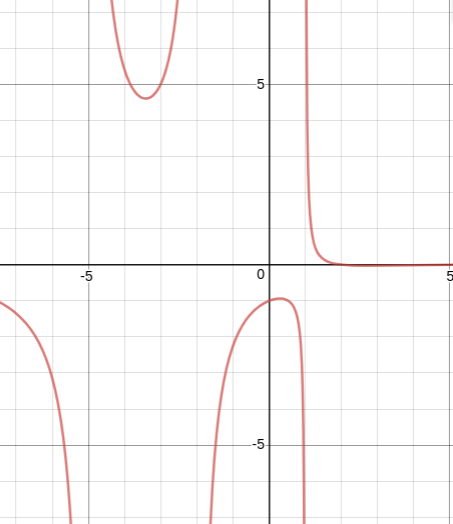
\includegraphics[width=0.5\textwidth]{../Figures/identifyGraphOfRationalFunctionC.png}
\end{center}
} \newpage
\item{
Write an equation of a function that \textit{could} be represented by the graph below. Explain why your function could represent the graph.
\begin{center}
    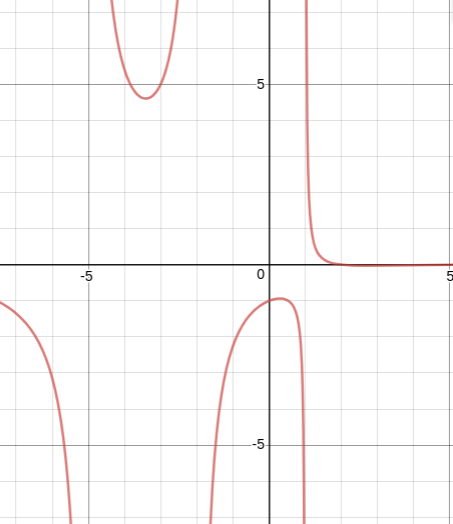
\includegraphics[width=0.5\textwidth]{../Figures/identifyGraphOfRationalFunctionCopyC.png}
\end{center}
} \newpage
\item{
Determine the horizontal and/or oblique asymptotes in the rational function below.\[ f(x) = \frac{6x^{3} -29 x^{2} +23 x + 30}{3x^{2} -13 x -10} \]} \newpage
\item{
Determine the vertical asymptotes and holes in the rational function below.\[ f(x) = \frac{12x^{3} -59 x^{2} +95 x -50}{9x^{2} -25} \]} \newpage
\item{
Determine the vertical asymptotes and holes in the rational function below.\[ f(x) = \frac{9x^{3} +15 x^{2} -2 x -8}{9x^{2} -18 x + 8} \]} \newpage
\item{
Determine the vertical asymptotes and holes in the rational function below.\[ f(x) = \frac{6x^{3} +49 x^{2} +125 x + 100}{9x^{2} +27 x + 20} \]} \newpage
\item{
Determine the horizontal and/or oblique asymptotes in the rational function below.\[ f(x) = \frac{6x^{3} +13 x^{2} -9 x -10}{3x^{2} -10 x -8} \]} \newpage
\end{enumerate}

\end{document}